\subsection{Grafik-Rendering-Pipeline}
\label{grp-rendering-pipeline}
Die Grafik-Rendering-Pipeline (\acrshort{grafik-rendering-pipeline}) dient dazu die dreidimensionalen Objekte mit einer virtuellen Kamera auf ein zweidimensionales Bild zu \textit{rendern}\footnote{\glqq ein Bild (eine Grafik) aus Rohdaten ([..] aus einer 3D-Szene[..]) durch einen Webbrowser/ein Programm erzeugen.\grqq{} https://de.wiktionary.org/wiki/rendern}.
Es handelt sich um eine Pipeline (Befehlskette), die aus mehreren Teilaufgaben bestehen. Die Geometrie, die Charakteristiken der Umgebung und die Platzierung der virtuellen Kamera in der Szene beeinflussen die Lokalisierung und die Form der 3D-Objekte. Die \acrshort{Materials}, \textit{Texturen}, Lichtquellen und Shader beeinflussen die Erscheinung \cite*[Moeller (2019)]{moeller2019}. Materials affektieren das Aussehen eines 3D Objekts mit Texturen, Farben oder der Eigenschaften von Reflexionen. Texturen sind Bilder, die die Oberfläche des Objekts benetzen. Abbildung \ref*{fig:renderpipeline1} zeigt mehrere dreidimensionale Objekte, die virtuelle Kamera und das daraus generierte zweidimensionale Bild. 

\begin{figure}[H]
    \centering
    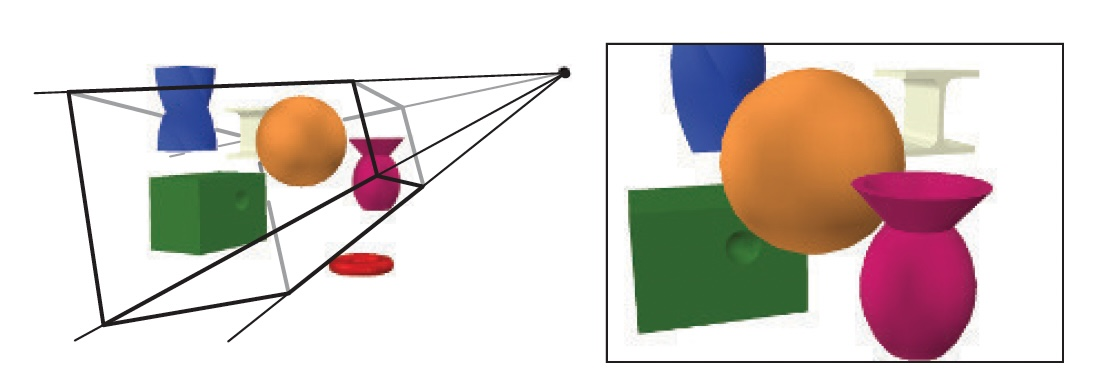
\includegraphics[width=\textwidth]{img/Render/render_pipeline_1.jpg}
    \caption{Die dreidimensionale Szene (links) und die zweidimensionale Sicht der virtuellen Kamera. Wird das Objekt perspektivisch gerendert, gibt es ein Raumvolumen (frustum). Es werden nur die Objekte gerendert, die sich innerhalb dieses Volumens befinden. So wird der rote Donut nicht und das blaue Objekt abgeschnitten dargestellt\cite*[Moeller (2019)]{moeller2019}.}
    \label{fig:renderpipeline1}
\end{figure}

Die \acrshort{grafik-rendering-pipeline} wird in vier Hauptstufen unterteilt: 

\begin{itemize}
    \item Applikation,
    \item Geometrieverarbeitung,
    \item Rasterisierung,
    \item Pixelverarbeitung.
  \end{itemize}

\begin{figure}[H]
    \centering
    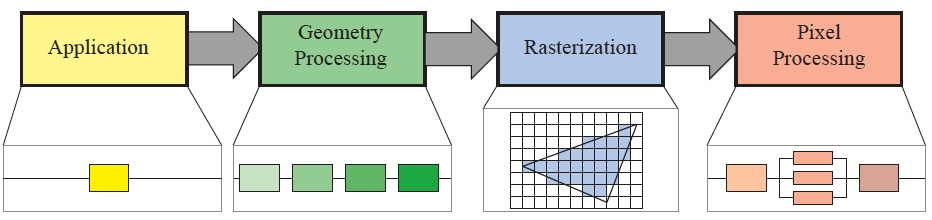
\includegraphics[width=\textwidth]{img/Render/render_pipeline_2.jpg}
    \caption{Die Basis der \acrshort{grafik-rendering-pipeline}, die in weitere Sub-Pipelines eingeteilt und parallel ausgeführt werden können \cite*{moeller2019}.}
    \label{fig:renderpipeline2}
\end{figure}

Die Abarbeitung der Aufgaben in den verschiedenen Stufen wird parallel ausgeführt. Durch die Parallelisierung ist eine verbesserte Performance möglich, da nicht jeder Prozess Schritt für Schritt durchgeführt werden muss. Jede Stufe kann gleichzeitig eine weitere Sub-Pipeline benutzen. So hat die Stufe \textit{Geometrieverarbeitung} in der Abbildung \ref*{fig:renderpipeline2} die Aufgabe in eine Sub-Pipeline gegliedert, die wiederum parallel ausgeführt werden kann. Die render Geschwindigkeit wird in \textit{frames pro sekunde} (\acrshort{frames-per-second}) angegeben und repräsentiert die Anzahl an Bilder, die pro Sekunde gerendert werden\cite*[Moeller (2019)]{moeller2019}. 

\subsubsection{Applikationsstufe}
Die Hauptaufgabe der Appliaktionsstufe besteht darin die benötigten Daten in die Pipeline zu schicken und zu aktualisieren. Die Daten bestehen aus den Render-Primitiven, die beispielsweise Punkte, Linien, Dreiecke oder Polygone (Vielecke) darstellen. Am Ende der Applikationsstufe werden die Rendering-Primitive an die Geometrieverarbeitungsstufe weitergegeben. Weiterhin finden Interaktionen wie z.B. Kollisionsabfragen statt oder es werden Input-Daten von Maus und Tastaur verarbeitet. Auch werden Culling-Algorithmen\footnote{ein Algorithmus, bei dem bestimmte (z.B. verdeckte) Polygone nicht gerendert werden, um eine bessere Performance zu erzielen \cite*{coorg1997}.} ausgeführt. Die Applikationsstufe wird im Gegensatz zu den anderen Stufen meist auf der \acrshort{cpu} ausgeführt. Entwickler haben dadurch eine hohe Kontrolle über die Prozesse in dieser Stufe. Sie können die Implementierung selbst bestimmen und im nachhinein modifizieren, um z.B. die Performance weiter zu verbessern\cite*[Moeller (2019)]{moeller2019}.

\subsubsection{Geometrieverarbeitung}
Auf dieser Stufe finden Operationen an den Polygonen und Vertices (Eckpunkte) statt. Sie wird auf der \acrshort{gpu} ausgeführt und lässt sich in eine Sub-Pipeline in Vertex-Shading, Projektion, Clipping und Window-Viewport-Transformation unterteilen.

\subsubsubsection{Vertex-Shading}
\label{grp-geometrieverarbeitung-vertex-shading}
Ein Vertex-Shader ist ein programmierbarer Shader in der Rendering-Pipeline, der die Eigenschaften jedes einzelnen Vertex bestimmt. Ein Vertex beinhaltet die Koordinaten von Punkten im dreidimensionalen Raum. Mithilfe von Informationen, welche Vertices miteinander verbunden sind, werden Linien und Polygone definiert \cite*[Vgl. Nischwitz (2012) S.48.]{nischwitz2012}. Die Aufgabe des Vertex-Shaders ist es, die Modellkoordinaten der Vertices durch Translation, Rotation oder Skalierung zu transformieren, um die Modelle zunächst im Weltkoordinatensystem, dann im Kamerakoordinatensystem und zuletzt im Clipping-Koordinatensystem zu lokalisieren. Die Transformationen werden mit 4x4 Transformtionsmatrizen durchgeführt. Der Vertex-Shader berechnet die Position eines Vertex von seinem Modellkoordinatensystem zum Clipping-Koordinatensystem:

\begin{equation}
    p'=P*K*W*p
    \label{vertex-transformationen}
\end{equation}
wobei:
\begin{conditions*}
    p'  &   Vertex in Clip-Koordinaten\\
    P   &   Projektionsmatrix \\
    K   &   Kamera-Transformation \\
    W   &   Welt-Transformation\\
    p   &   Vertex in Modellkoordinaten
\end{conditions*}

Die Reihenfolge der Transformationen spielt eine wichtige Rolle, da die Matrizenmultiplikation nicht kommutativ ist. Die Transformationen in der Gleichung \ref*{vertex-transformationen} müssen daher von rechts nach links durchgeführt werden.

Die Vertices der Modelle befinden sich ursprünglich in ihrem eigenen Modellkoordinatensystem. Die Szene hat ein Weltkoordinatensystem und ein Kamerakoordinatensystem. Die Vertices werden zunächst in das Weltkoordinatensystem transformiert. Die Kamera in der Szene hat Koordinaten im Weltkoordinatensystem und eine Richtung, in die die Kamera zeigt. Mit der Kamera-Transformation werden die Vertices und die Kamera so platziert, dass die Kamera in der Position des Ursprungs des Weltkoordinatensystems liegt und (meist) in negativer z-Richtung zeigt, während die y-Achse nach oben und die x-Achse nach rechts zeigt. Die genaue Definition der Richtungen der Koordinatenachsen hängt von der jeweiligen Anwendung ab. Das daraus folgende Koordinatensystem wird Kamerakoordinatensystem genannt. Somit befinden sich die Vertices nach den Kamera-Transformationen im Kamerakoordinatensystem. Schließlich wird eine Projektionsmatrix angewandt, um die Kamerakoordinaten der Vertices in Clipping-Koordinaten zu transformieren.

Zusätzlich zu den Transformationen bestimmt ein Vertex-Shader Eigenschaften wie die Farbe, Texturkoordinaten oder Normalenvektoren für jeden Vertex. Diese beschreiben das Material des Objekts und Effekte von Lichtquellen, die auf die Oberfläche scheinen. Die Wirkung von Licht auf ein Material wird Shading genannt. Es werden "[..]Normalenvektoren und Materialeigenschaften der Objekte auf der einen Seite und den Eigenschaften der Lichtquellen auf der anderen Seite für jeden Vertex die Beleuchtungsrechnung durchgeführt und somit eine Farbe ermittelt" \cite*[Nischwitz (2012) S.48,][]{nischwitz2012}. Die Ergebnisse der Berechnungen werden zur Rasterisierung und zur Pixelverarbeitung weitergeschickt\cite*[Moeller (2019)]{moeller2019}.

Mit Vertex-Shadern ist es möglich Oberflächen realistisch darzustellen, ohne die Polygonanzahl zu erhöhen. So nutzen Mitchell\cite*[][]{mitchell2005} und Isidoro \cite*[][]{isidoro2002} Vertex-Shader, um mit Heightmaps %Link und Kapitel Heightmaps
und Normalmaps %Link und Kapitel Normalmaps
einen realistischen Ozean zu rendern.

\subsubsubsection{Projektion}
\label{grp-geometrieverarbeitung-projektion}
Bei der Projektion werden zwei Aufgaben durchgeführt. Zum einen wird ein Clipspace (Kanonisches-Sichtvolumen) definiert, das meist in Form eines Einheitswürfels\footnote{ein Würfel mit der Skalierung (1,1,1)} gegeben ist. Der Würfel ist für das Clipping von Bedeutung.

Zum anderen wird eine Projektionsmethodik je nach Anwendungsfall bestimmt. Beispielsweise gibt es eine orthographische Projektion, bei der parallele Linien auch parallel erscheinen, während bei der perspektivischen Projektion parallele Linien Fluchtpunkten folgen. Die Projektionsmethodik bestimmt die Projektionsmatrix für die Transformation in die Clipping-Koordinaten.

\subsubsubsection{Clipping}
\label{grp-geometrieverarbeitung-clipping}
Nur mit den im Vertex-Shader transformierten Clipping-Koordinaten der Vertices kann Clipping durchgeführt werden. Es werden nur die Primitiven zur Window-Viewport-Transformation weitergeschickt, die sich innerhalb des kanonischen-Sichtvolumens befinden. Clipping wird dann benötigt, wenn sich ein Teil eines Primitiven innerhalb und ein anderer Teil außerhalb des Sichtvolumens befinden. Die Primitiven, die sich mit dem Einheitswürfel schneiden, erhalten an der Schnittkante neue Vertices\cite*[Moeller (2019)][]{moeller2019}.

\subsubsubsection{Window-Viewport-Transformation}
\label{grp-geometrieverarbeitung-window-viewport-transformation}
Im nächsten Schritt wird mit den Primitiven eine Window-Viewport-Transformation durchgeführt. Dadurch wird es möglich die x- und y-Koordinaten der Primitiven auf ein Bildschirmausschnitt (Viewport) darzustellen. Die Primitiven erhalten Bildschirm- bzw. Window-Koordinaten\footnote{Bildschirm-Koordinaten sind zweidimensionale (x,y)-Koordinaten, während Window-Koordinaten auch die z-Koordinate beinhaltet (x,y,z).}. Es handelt sich dabei um eine Translation gefolgt von einer Skalierung\cite*[Moeller (2019) S.20f.,][]{moeller2019} \cite*[Nischwitz (2012) S.150,][]{nischwitz2012}.

\subsubsection{Rasterisierung}
\label{grp-rasterisierung}
Bei der Rasterisierung werden mit einer perspektivischen Projektion Pixel gesucht, die sich auf dem Viewport innerhalb der gerenderten Primitiven befinden. Es findet eine Übersetzung der 3D-Koordinaten in 2D-Pixelkoordinaten statt. Klassische Rasterisierungs-Algorithmen definieren einen zugehörigen Pixel genau dann, wenn ein Pixel sich innerhalb eines Primitiven befindet. Es werden sogenannte \textit{Fragmente} für den Teil des Pixels erzeugt, der sich mit dem Dreieck überschneidet\cite*[][, zuletzt aufgerufen am 11.07.2022]{scratchapixel} cite*[Moeller (2019) S.21f.,][]{moeller2019}. 

\begin{figure}[hbt!]
    \centering
    \subfloat[][]{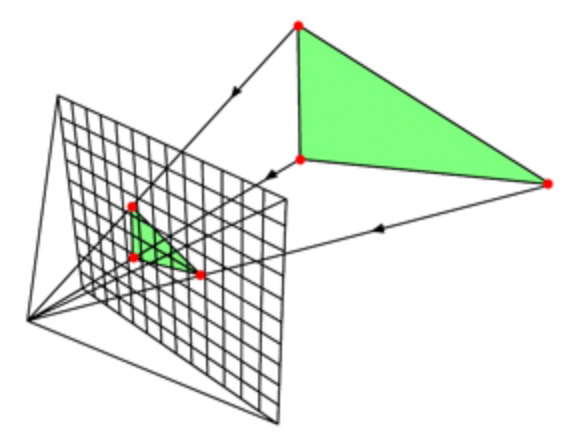
\includegraphics[width=0.4\linewidth]{img/Render/rasterisierung_1.jpg}}%
    \qquad
    \subfloat[][]{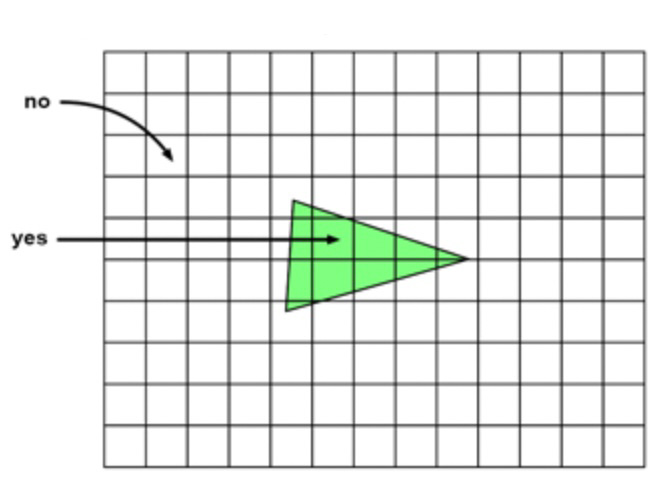
\includegraphics[width=0.4\linewidth]{img/Render/rasterisierung_2.jpg}}%
    \caption{Die Primitiven werden in eine 2D-Ebene projiziert(a). Befindet sich ein Pixel innerhalb des Primitiven, werden diskrete Fragmente gebildet, die im in der Pixelverarbeitung weitergeschickt werden(b) \cite*[][, zuletzt aufgerufen am 11.07.2022]{scratchapixel}.}%
    \label{fig:rendering-pipeline-rasterisierung-beispiel}
\end{figure}

\subsubsection{Pixelverarbeitung (Fragment-Shader)}
\label{grp-pixelverarbeitung}
Bei der Pixelverarbeitung werden die diskreten Fragmente aus der Rasterisierung mit einem Fragment-Shader verarbeitet. So werden im einfachsten Fall die endgültigen Farben der Fragmente festgelegt oder auch Texturen an das Modell angeheftet. 
%Eigenes Beispiel mit gescheiten Outline Shader zeigen!

Nach dem Fragment-Shader wird überprüft, ob sich im dreidimensionalen Raum zwei oder mehrere Fragmente überlappen. Für diesen Fall gibt es einen z-Buffer, der für jedes Fragment einen z-Wert gespeichert hat. Dieser z-Wert repräsentiert wie weit das Fragment von der Kamera entfernt ist. Ein z-Buffer Algorithmus entscheidet dann, welches Fragment näher zur Kamera liegt und welche Farbe das Fragment letzendlich haben soll. Dieser Algorithmus ist simpel und hat den Vorteil, dass die render Reihenfolge der Primitiven trivial ist. Probleme gibt es jedoch bei transparenten Objekten. Hier ist die Reihenfolge für eine korrekte Darstellung wichtig\cite*[Moeller (2019) S.21f.,][]{moeller2019}. Für eine ausführliche Erklärung für den Umgang mit transparenten Objekten wird auf Möller, Kapitel 5.5 verwiesen\cite*[Moeller (2019) S.148ff.,][]{moeller2019}.